\documentclass[11pt,aspectratio=1610,xcolor=dvipsnames]{beamer}

\usetheme[
    background=light,
    numbering=fraction,
    block=fill,
    progressbar=frametitle
]{metropolis}

\graphicspath{{img/}}

\usepackage[style=authortitle-ibid,backend=biber]{biblatex}
\addbibresource{refs.bib}
\setbeamerfont{footnote}{size=\scriptsize}

\usepackage{physics}
\usepackage{mathtools}
\usepackage{bbm}
\usepackage{booktabs}
\usepackage[most,skins,theorems]{tcolorbox}
\tcbset{variables/.style={colback=yellow!20,colframe=yellow}}
\usepackage{tikz}
\usetikzlibrary{shapes.geometric, arrows, shadows}
\usetikzlibrary{fit, backgrounds}



% \colorlet{LightLavender}{Lavender!40!}
\newtcolorbox{prob}{colback=red!5!white,colframe=red!75!black}
\usefonttheme[onlymath]{serif}
\usepackage{quantikz}
\usepackage{qrcode}
\usepackage{pgfplots}
\usepackage{pythonhighlight}

\newcommand{\R}{\mathbb{R}}
\newcommand{\U}[1]{\mathsf{U}(#1)}
\newcommand{\defeq}{\stackrel{\text{\tiny def}}{=}}

\titlegraphic{
\includegraphics[width=0.3\textwidth]{unitary_fund_logo.png}}

\title{Richardson Extrapolation}
\subtitle{Quantum Wednesday}
\date{Feb 8, 2023}
\author{Nate Stemen}


\begin{document}

\maketitle

\begin{frame}{Today's Paper}
	\begin{figure}[h]
		\centering
		
\includegraphics[width=0.9\textwidth]{abstract.png}
	\end{figure}
	\begin{center}
		\url{https://arxiv.org/abs/2201.08080}
	\end{center}
\end{frame}

\begin{frame}{Overview}
	\begin{enumerate}
		\item What is Richardson Extrapolation?
		\item How do we \emph{already} use it?
		\item What sort of optimizations do the authors find?
	\end{enumerate}
\end{frame}

\begin{frame}{What is extrapolation?}

\end{frame}

\begin{frame}[fragile]{How do we use Richardson Extrapolation?}
	% \begin{noindent}
	\begin{python}
		class RichardsonFactory():
			def extrapolate(
				scale_factors: Sequence[float],
				exp_values: Sequence[float],
				full_output: bool = False,
			) -> ExtrapolationResult:
				# Richardson extrapolation is a particular case of a
				# polynomial fit with order equal to the number of
				# data points minus 1.
				order = len(scale_factors) - 1
				return PolyFactory.extrapolate(
					scale_factors, exp_values, order, full_output
				)
	\end{python}
	% \end{noindent}
\end{frame}

\begin{frame}{Problem setup}
	\begin{columns}
		\begin{column}{0.5\textwidth}
			\begin{itemize}
				\item $E(\lambda) = \tr(\rho_\lambda A)$
				\item $\lim_{\lambda\to 0}E(\lambda) = E^*$
				\item Define $\lambda = \lambda_0 x$, and assume we can access any $x \geq 1$
				\item Take $1 = x_0 < x_1 < \cdots < x_n$, and collect $E(x_i)$
				\item Interpolate a polynomial of degree $n$ to $(x_i, E(x_i)$)
				\item Evaluate polynomial at $\lambda = 0$
			\end{itemize}
			\begin{align*}
				E(0)     & \approx \sum_{i = 0}^n E(x_i)\gamma_i =: R_n \\
				\gamma_i & = \prod_{k \neq j}\frac{x_k}{x_k - x_j}
			\end{align*}
		\end{column}
		\begin{column}{0.5\textwidth}
			\begin{align*}
				E(x) & = E^* + \sum_{k = 0}^\infty a_k \lambda_0^k x^k                                                  \\
				E(0) & \approx \sum_{i = 0}^n\qty[E^* + \sum_{k = 0}^\infty a_k\lambda_0^k x_i^k]\gamma_i               \\
				     & = E^* \sum_{i = 0}^n \gamma_i + \sum_{i = 0}^n\sum_{k = 0}^\infty a_k \lambda_0^k \gamma_i x_i^k \\
				     & = E^* + \sum_{k = n+1}^\infty a_k\lambda_0^k \; \sum_{i = 0}^n \gamma_i x_i^k
			\end{align*}
		\end{column}
	\end{columns}
\end{frame}

\begin{frame}{Bias and Variance}

	\begin{columns}
		\begin{column}{0.7\textwidth}
			\begin{align*}
				\mathrm{Bias}[\hat{R}_n]   & = (-1)^n E^{(n+1)}(\xi)\frac{C_n}{(n+1)!}        \\
				\mathrm{Var}[\hat{E}(x_i)] & = \frac{\sigma_i^2}{N_i}                         \\
				\mathrm{Var}[\hat{R}_n]    & = \sum_{i = 0}^n \gamma_i^2 \frac{\sigma^2}{N_i}
			\end{align*}
		\end{column}
		\begin{column}{0.3\textwidth}
			\begin{align*}
				C_n      & = \prod_{i = 0}^n x_i                           \\
				\xi      & \in [0, x_n]                                    \\
				\sigma_i & = \sqrt{\tr(\rho_{\lambda_0x_i}A^2) - E(x_i)^2} \\
				N_i      & = \text{\# times $A$ is measured at $x_i$}
			\end{align*}
		\end{column}
	\end{columns}

\end{frame}

\begin{frame}{What could we optimize?}
	\begin{enumerate}
		\item Is there a way to reduce the increase in variance?
		\item Is there a scaling method for the $x_i$'s that optimizes the bias/variance tradeoff?
		\item Is there an optimal number of samples $n$?
	\end{enumerate}
\end{frame}

\begin{frame}{Variance reduction}
	A \textbf{simple} calculation shows $\mathrm{Var}[\hat{R}_n] = \sum_{i = 0}^n \gamma_i^2 \frac{\sigma^2}{N_i}$ is minimized by
	\begin{equation*}
		N_i = N_\text{total}\frac{\abs{\gamma_i}}{\sum_{k = 0}^n \abs{\gamma_k}}
	\end{equation*}

	Defining $\Lambda = \sum_{i = 0}^n \abs{\gamma_i}$ and $N_\text{eff} = N_\text{total} / \Lambda^2$:
	\begin{align*}
		\mathrm{Var}[\hat{R}_n] = \frac{\sigma^2}{N_\text{total}}\Lambda^2 = \frac{\sigma^2}{N_\text{eff}}
	\end{align*}
\end{frame}

\begin{frame}{Node Spacing}

	\begin{columns}
		\begin{column}{0.5\textwidth}
			\begin{align*}
				x_j^\mathrm{L} & = 1 + j(x_1 - 1)                                                                             \\
				x_j^\mathrm{E} & = x_1^j                                                                                      \\
				x_j^\mathrm{C} & = 1 + \frac{\sin^2(\frac{j}{n}\frac{\pi}{2})}{\sin^2(\frac{1}{n}\frac{\pi}{2})}(x_1 - 1)     \\
				x_j^\mathrm{T} & = 1 + \frac{\sin^2(\frac{j}{n+1}\frac{\pi}{2})}{\sin^2(\frac{1}{n+1}\frac{\pi}{2})}(x_1 - 1)
			\end{align*}
			\begin{figure}[h]
				\centering
				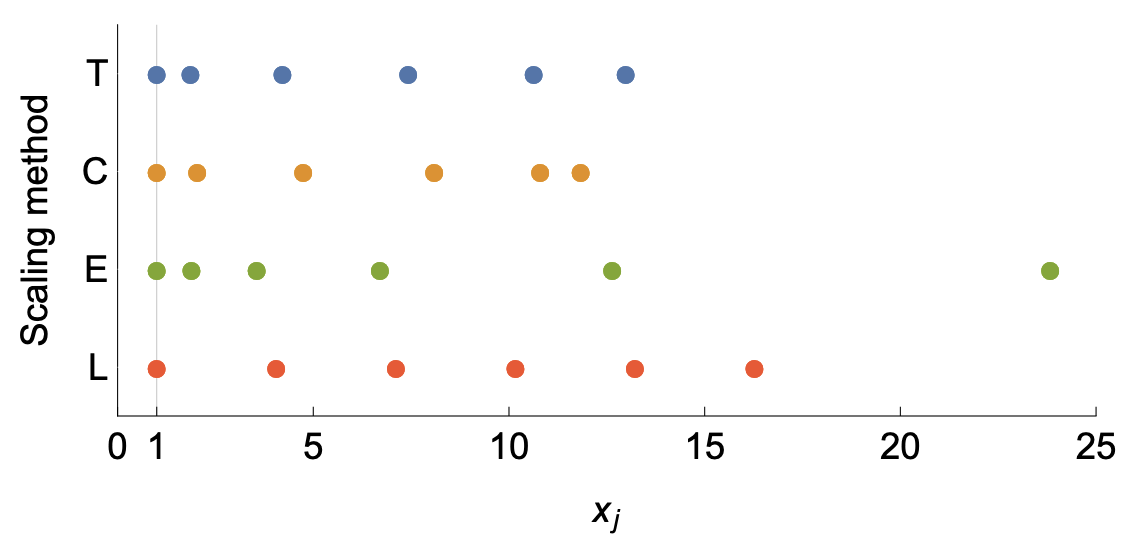
\includegraphics[width=\textwidth]{spacing.png}
			\end{figure}
		\end{column}
		\begin{column}{0.5\textwidth}
			\begin{figure}[h]
				\centering
				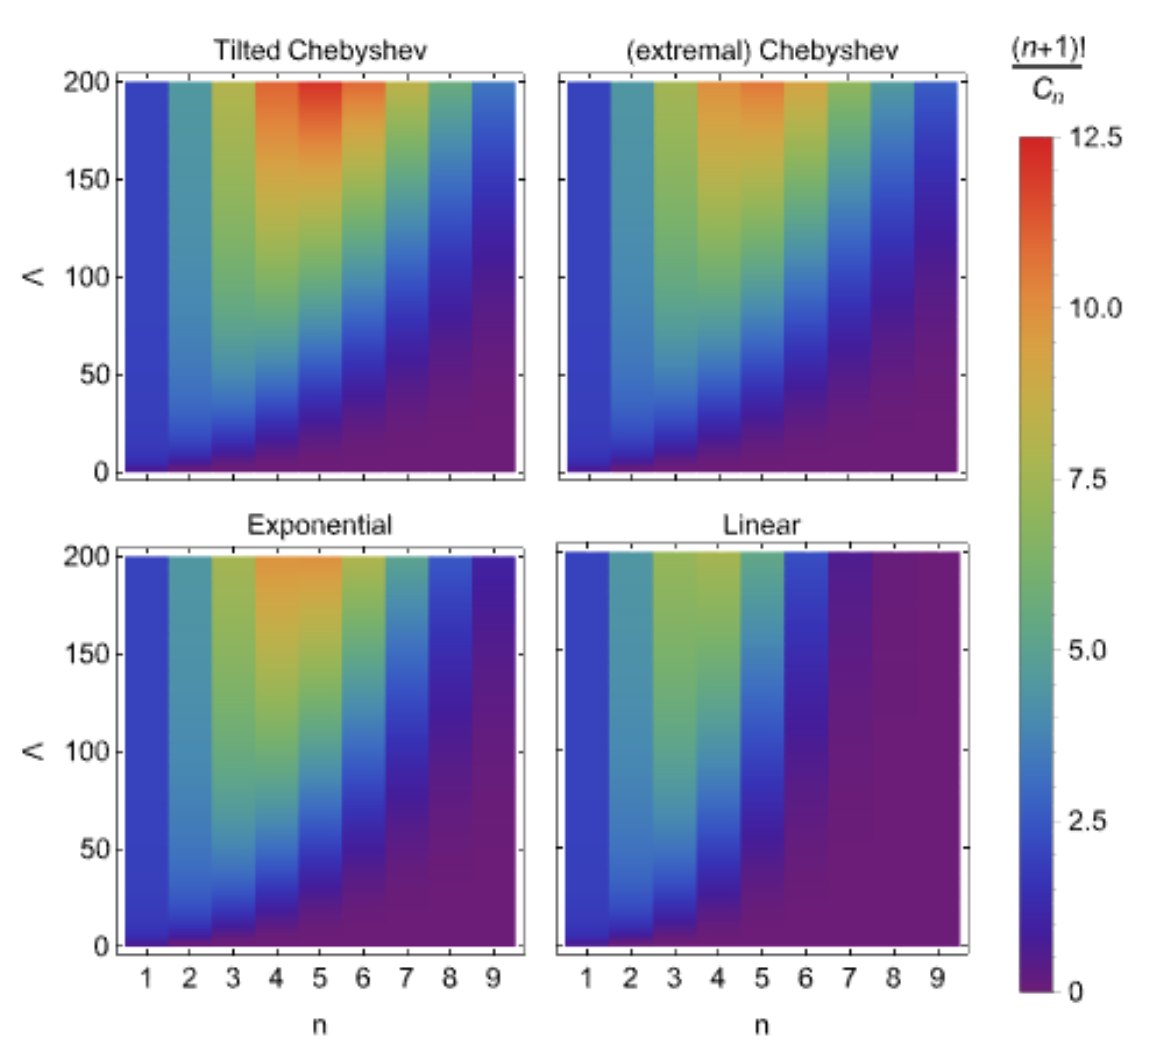
\includegraphics[width=\textwidth]{spacing-quality.png}
			\end{figure}
		\end{column}
	\end{columns}

\end{frame}

\begin{frame}{Overview}
	\begin{figure}[h]
		\centering
		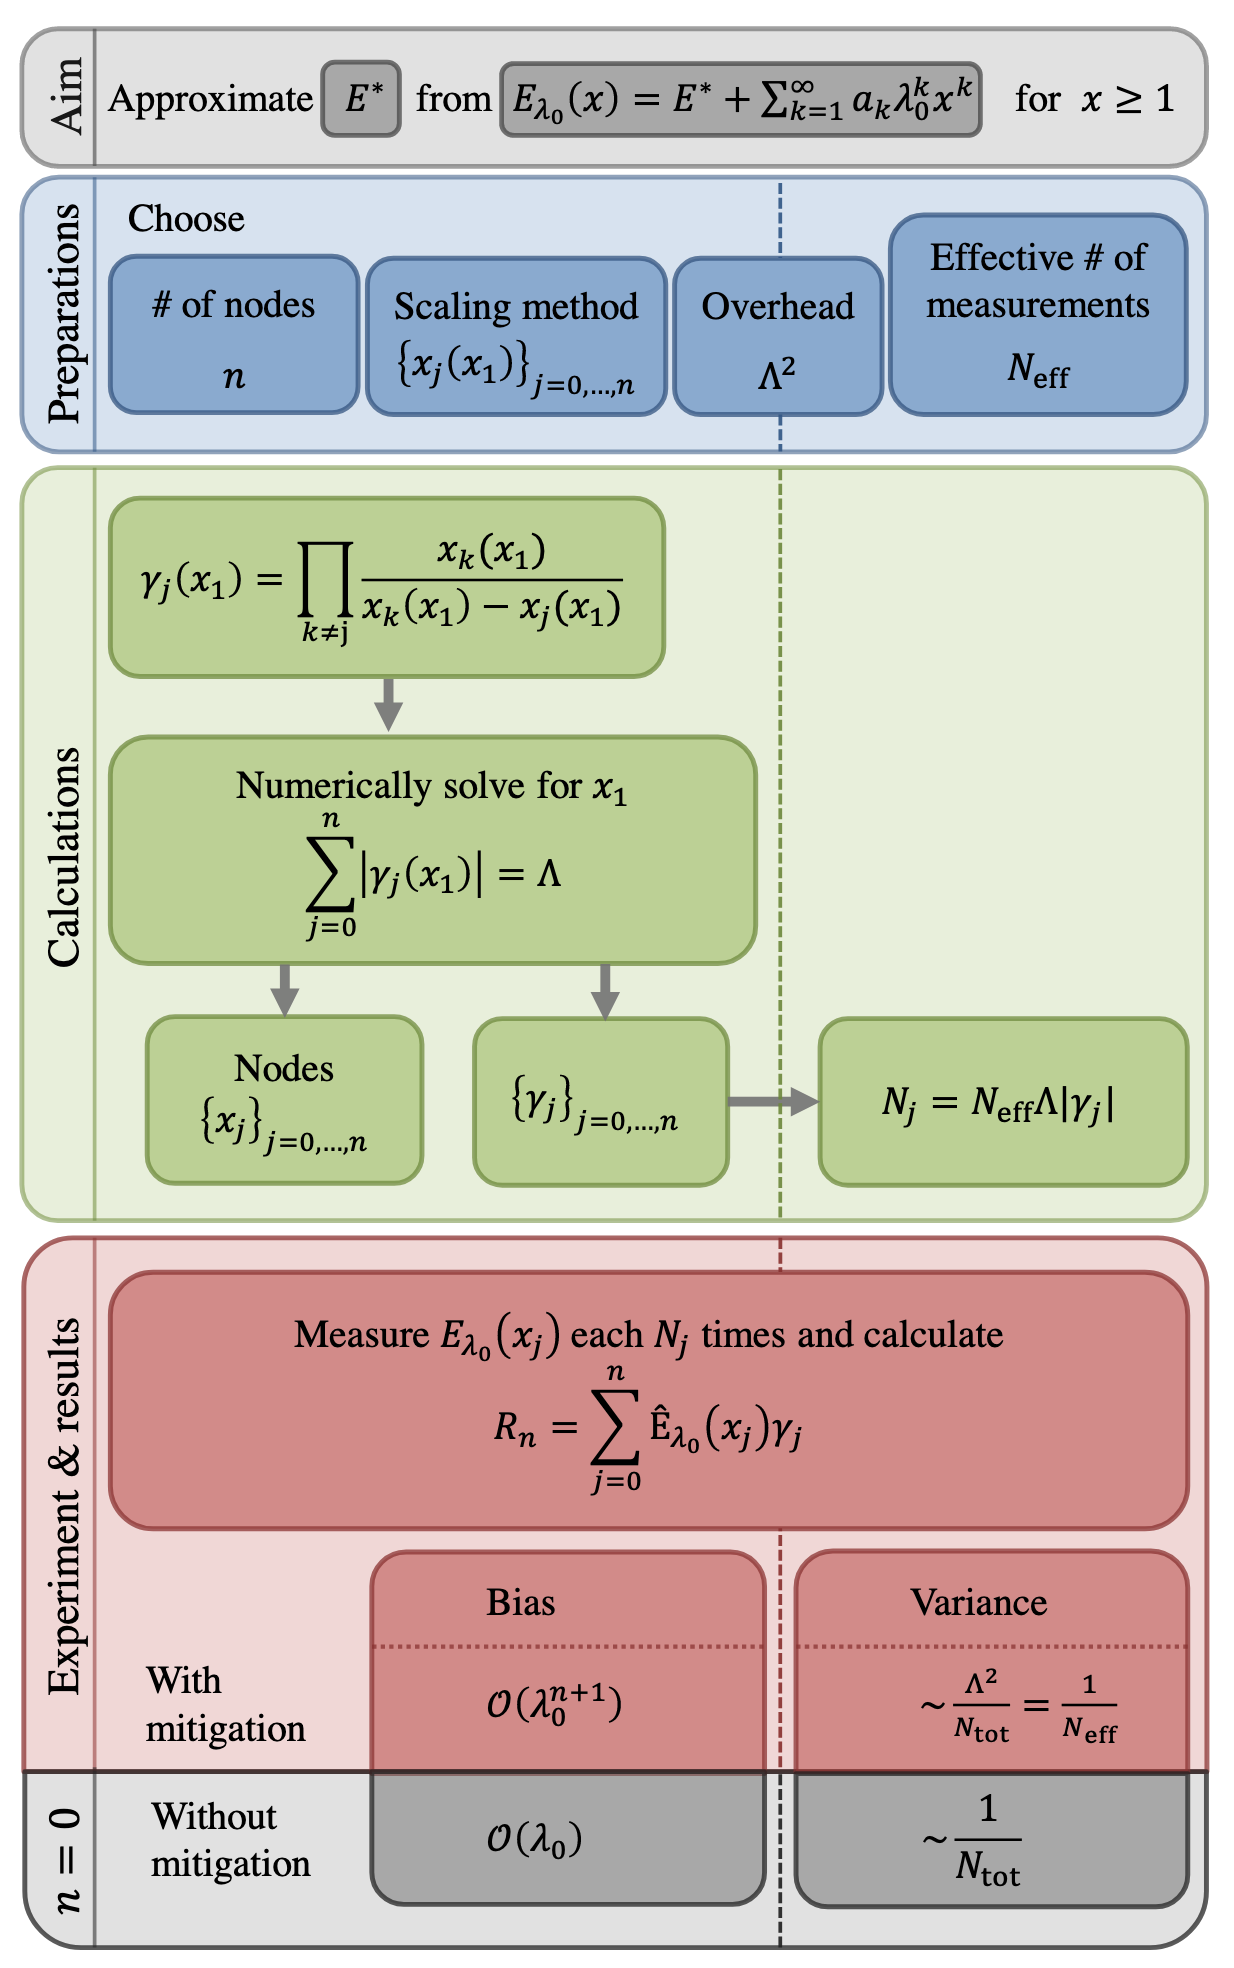
\includegraphics[height=0.95\textheight]{overview.png}
	\end{figure}
\end{frame}

\begin{frame}{Results}
	\begin{figure}[h]
		\centering
		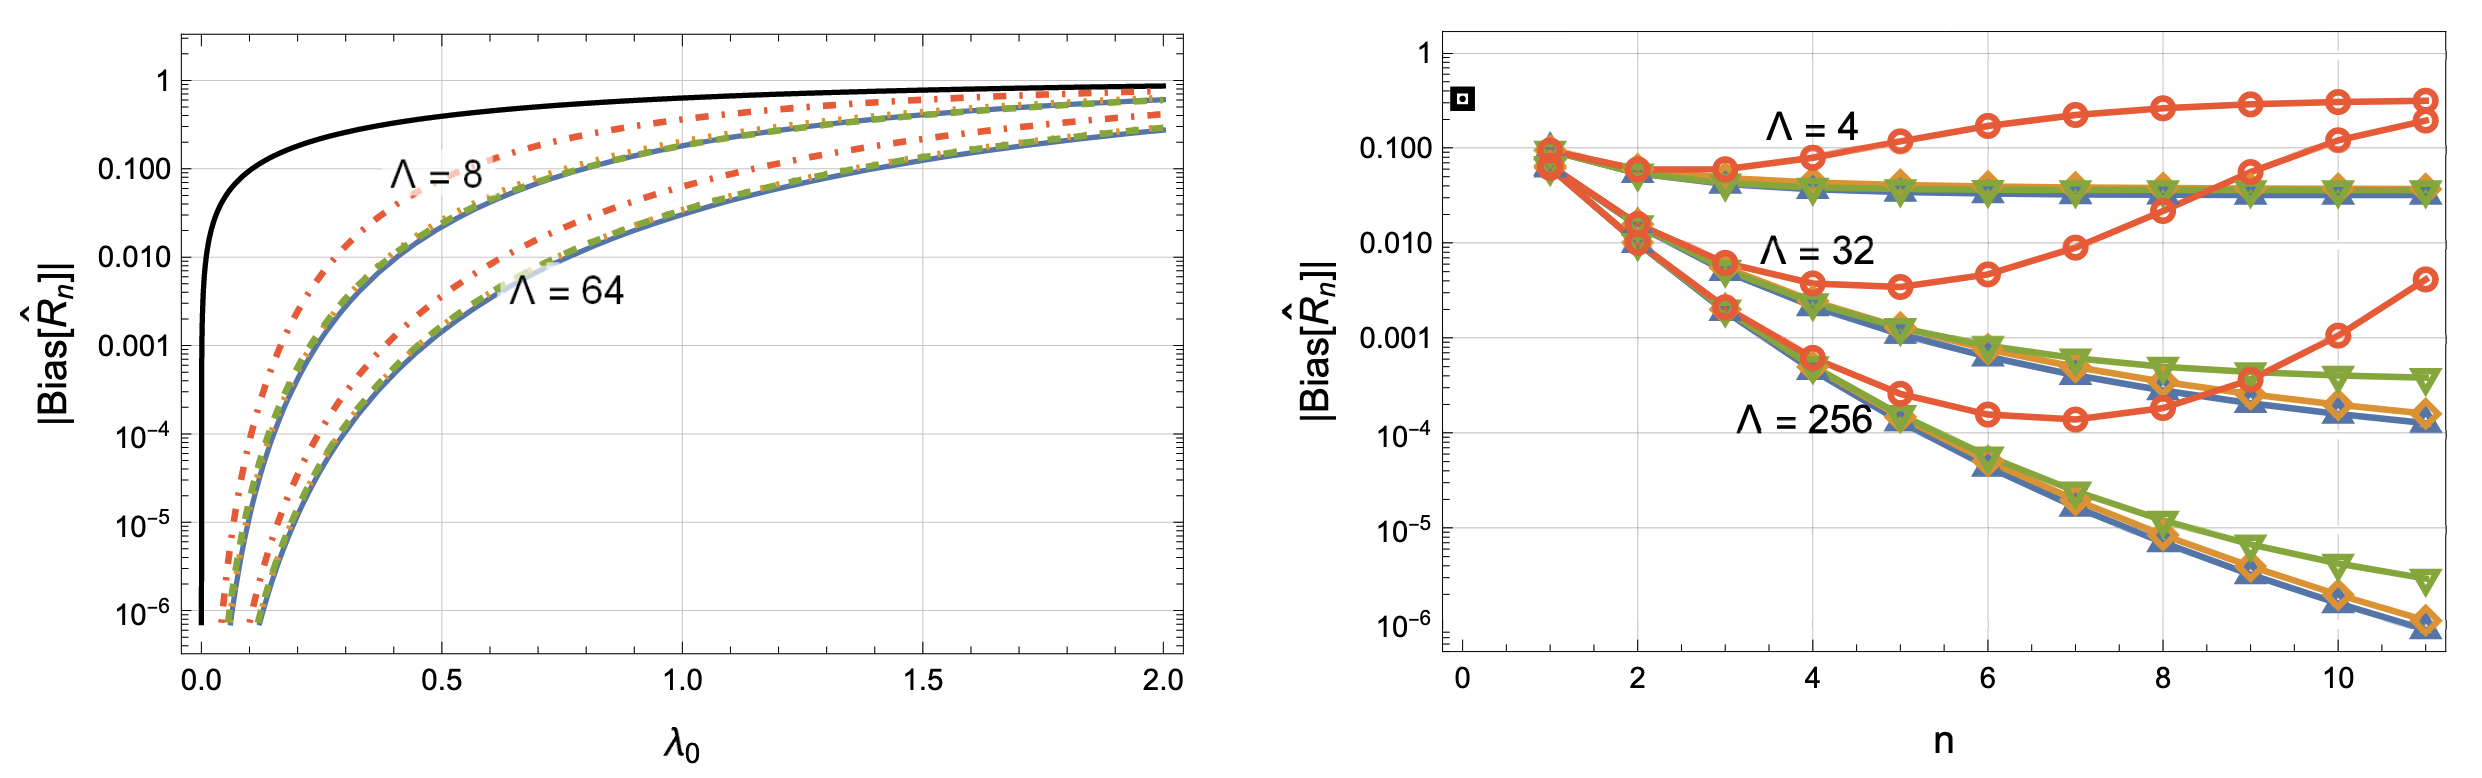
\includegraphics[width=0.9\textwidth]{results.png}
		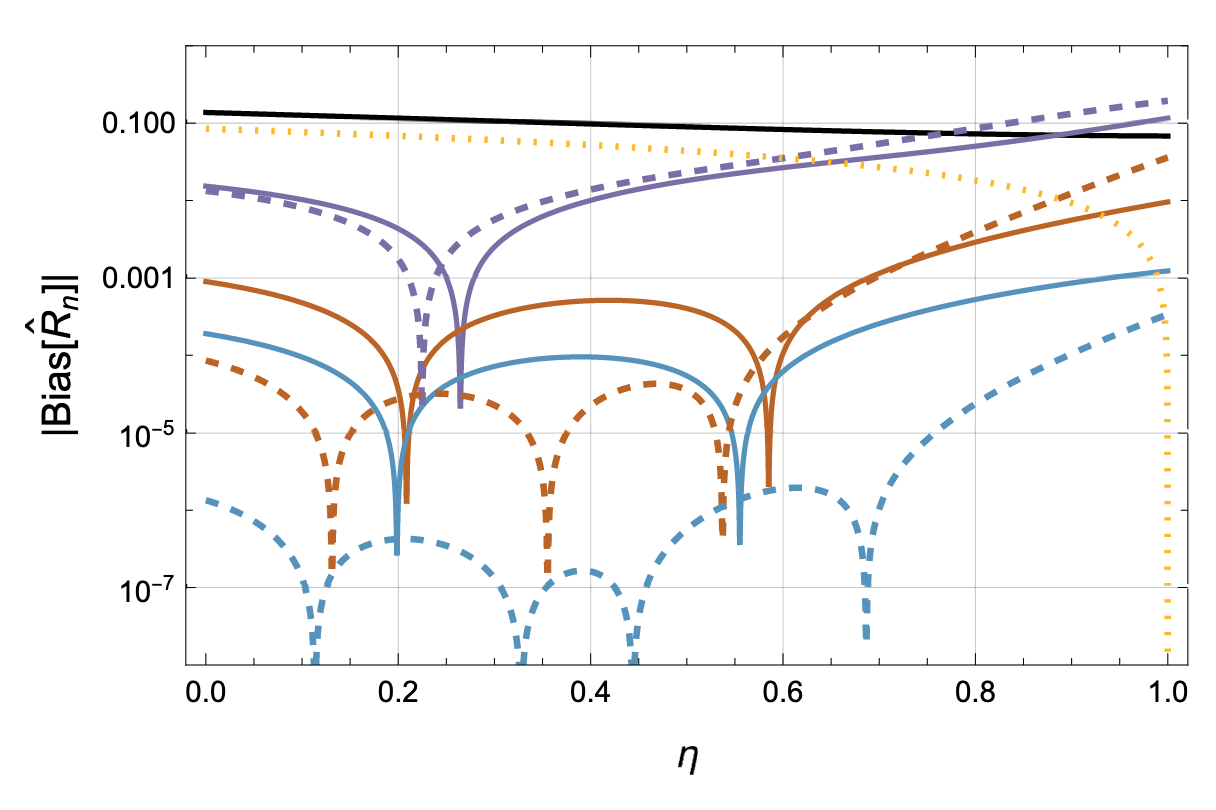
\includegraphics[width=0.5\textwidth]{markovianity.png}
	\end{figure}
\end{frame}

\begin{frame}[standout]
	Thank you!
\end{frame}

\end{document}
